\input slide_preamble
\input preamble

\begin{document}

{\Huge
  \centerline{\bf TTIC 31230,  Fundamentals of Deep Learning}
  \vfill
  \centerline{David McAllester, Autumn 2020}
  \vfill
\centerline{Some Information Theory}

\slide{Why Information Theory?}

The fundamental equation involves cross-entropy.

\vfill
Cross-entropy is an information-theoretic concept.

\vfill
Information theory arises in many places and many forms in deep learning.

\slide{Entropy of a Distribution}

The entropy of a distribution $P$ is defined by

\vfill
$${\color{red} H(P) = E_{y \sim \pop} \;- \ln P(y)}\;\;\mbox{in units of ``nats''}$$

\vfill
$${\color{red} H_2(P) = E_{y \sim \pop} \;- \log_2 P(y)}\; \mbox{in units of bits}$$

\slide{Why Bits?}

Why is $-\log_2\;P(y)$ a number of bits?

\vfill
Example: Let $P$ be a uniform distribution on 256 values.

\vfill
$$E_{y \sim P}\;-\log_2 P(y) = - \log_2 \frac{1}{256} = \log_2 256 = 8\;\mathrm{bits} = 1\;\mathrm{byte}$$

\vfill
\centerline{\color{red} 1 nat = $\frac{1}{\ln 2}$ bits $\approx$ 1.44 bits}

\slide{Shannon's Source Coding Theorem}

Why is $-\log_2\;P(y)$ a number of bits?

\vfill
A prefix-free code for ${\cal Y}$ assigns a bit string $c(y)$ to each $y \in {\cal Y}$ such that no code string is prefix of any other code string.

\vfill
For a probability distribution $P$ on ${\cal Y}$ we consider the average code length $E_{y \sim P} \;|c(y)|$.

\vfill
Theorem: For any $c$ we have {\color{red} $E_{y \sim P}\;|c(y)| \geq H_2(P)$}.

\vfill
Theorem: There exists $c$ with {\color{red} $E_{y \sim P} \;|c(y)| \leq H_2(P) +1$}.

\ignore{
For any bit string $c$ let $|c|$ be the number of bits in (the length of) $c$.
\vfill
Theorem: There exists a coding function $c(y)$ such that for all $y$
$$|c(y)| \leq (- \log_2\;P(y)) + 1$$
and therefore
$$E_y\;|c(y)| \leq H_2(y)+1$$

\vfill
Theorem: For any coding scheme $c$
$$E_y |c(y)| \geq H_2(y)$$
}

\slide{Cross Entropy}

Let $P$ and $Q$ be two distribution on the same set.

{\color{red} $$H(P,Q) = E_{y \sim P} \;-\ln \;Q(y)$$}

{\color{red} $$\Phi^* = \argmin_\Phi \;H(\pop,P_\Phi)$$}

\vfill
{\color{red} H(P,Q)} also has a data compression interpretation.

\vfill
{\color{red} $H(P,Q)$} can be interpreted as 1.44 times the number of bits used to code draws from $P$ when using the imperfect code defined by $Q$.

\slide{Entropy, Cross Entropy and KL Divergence}

Let $P$ and $Q$ be two distribution on the same set.

\vfill
\centerline{
  $\begin{array}{lrcl}
\mathrm{Entropy}: & {\color{red} H(P)} & = & {\color{red} E_{y \sim P}\;-\ln\;P(y)} \\
\\
\mathrm{Cross Entropy:} & {\color{red} H(P,Q)} & = & {\color{red} E_{y \sim P}\;-\ln\;Q(y)} \\
\\
\mathrm{KL\; Divergence:} & {\color{red} KL(P,Q)} & = & {\color{red} H(P,Q) - H(P)} \\
\\
& & = & {\color{red} E_{y \sim P}\;\;\; \ln\;\frac{P(y)}{Q(y)}}
\end{array}$}

\vfill
We have {\color{red} $H(P,Q) \geq H(P)$} or equivalently {\color{red} $KL(P,Q) \geq 0$}.

\slide{The Universality Assumption}

{\color{red} $$\Phi^* = \argmin_\Phi\;H(\pop,P_\Phi) = \argmin_\Phi\;H(\pop) + KL(\pop,P_\Phi)$$}

\vfill
Universality assumption: {\color{red} $P_\Phi$ can represent any distribution and $\Phi$ can be fully optimized.}

\vfill
This is clearly false for deep networks.  {\color{red} But it gives important insights like:}

{\color{red} $$P_{\Phi^*} = \pop$$}

\vfill
{\color{red} \centerline{This is the motivatation for the fundamental equation.}}


\slide{Asymmetry of Cross Entropy}
Consider 


$$\Phi^* = \argmin_\Phi \;H(P,Q_\Phi)\;\;\;\;\;(1)$$

\vfill
$$\Phi^* = \argmin_\Phi \;H(Q_\Phi,P)\;\;\;\;\;(2)$$

\vfill
For (1) $Q_\Phi$ must cover all of the support of $P$.

\vfill
For (2) $Q_\Phi$ concentrates all mass on the point maximizing $P$.

    
\slide{Asymmetry of KL Divergence}
Consider 


\begin{eqnarray*}
  \Phi^* & = & \argmin_\Phi \;KL(P,Q_\Phi) \\
  & = & \argmin_\Phi\; H(P,Q_\Phi)\;\;\;\;\;\;\;\;\;\;\;\;\;\;\;\;\;\;(1) \\
  \\
  \Phi^* & = & \argmin_\Phi \;KL(Q_\Phi,P) \\
  & = & \argmin_\Phi H(Q_\Phi,P) - H(Q_\Phi)\;\;\;(2)
  \end{eqnarray*}

\vfill
If $Q_\Phi$ is not universally expressive we have that (1) still forces $Q_\Phi$ to cover all of $P$ (or else the KL divergence is infinite)
while (2) allows $Q_\Phi$ to be restricted to a single mode of $P$ (a common outcome).

\slideplain{Proving $KL(P,Q) \geq 0$: Jensen's Inequality}

\centerline{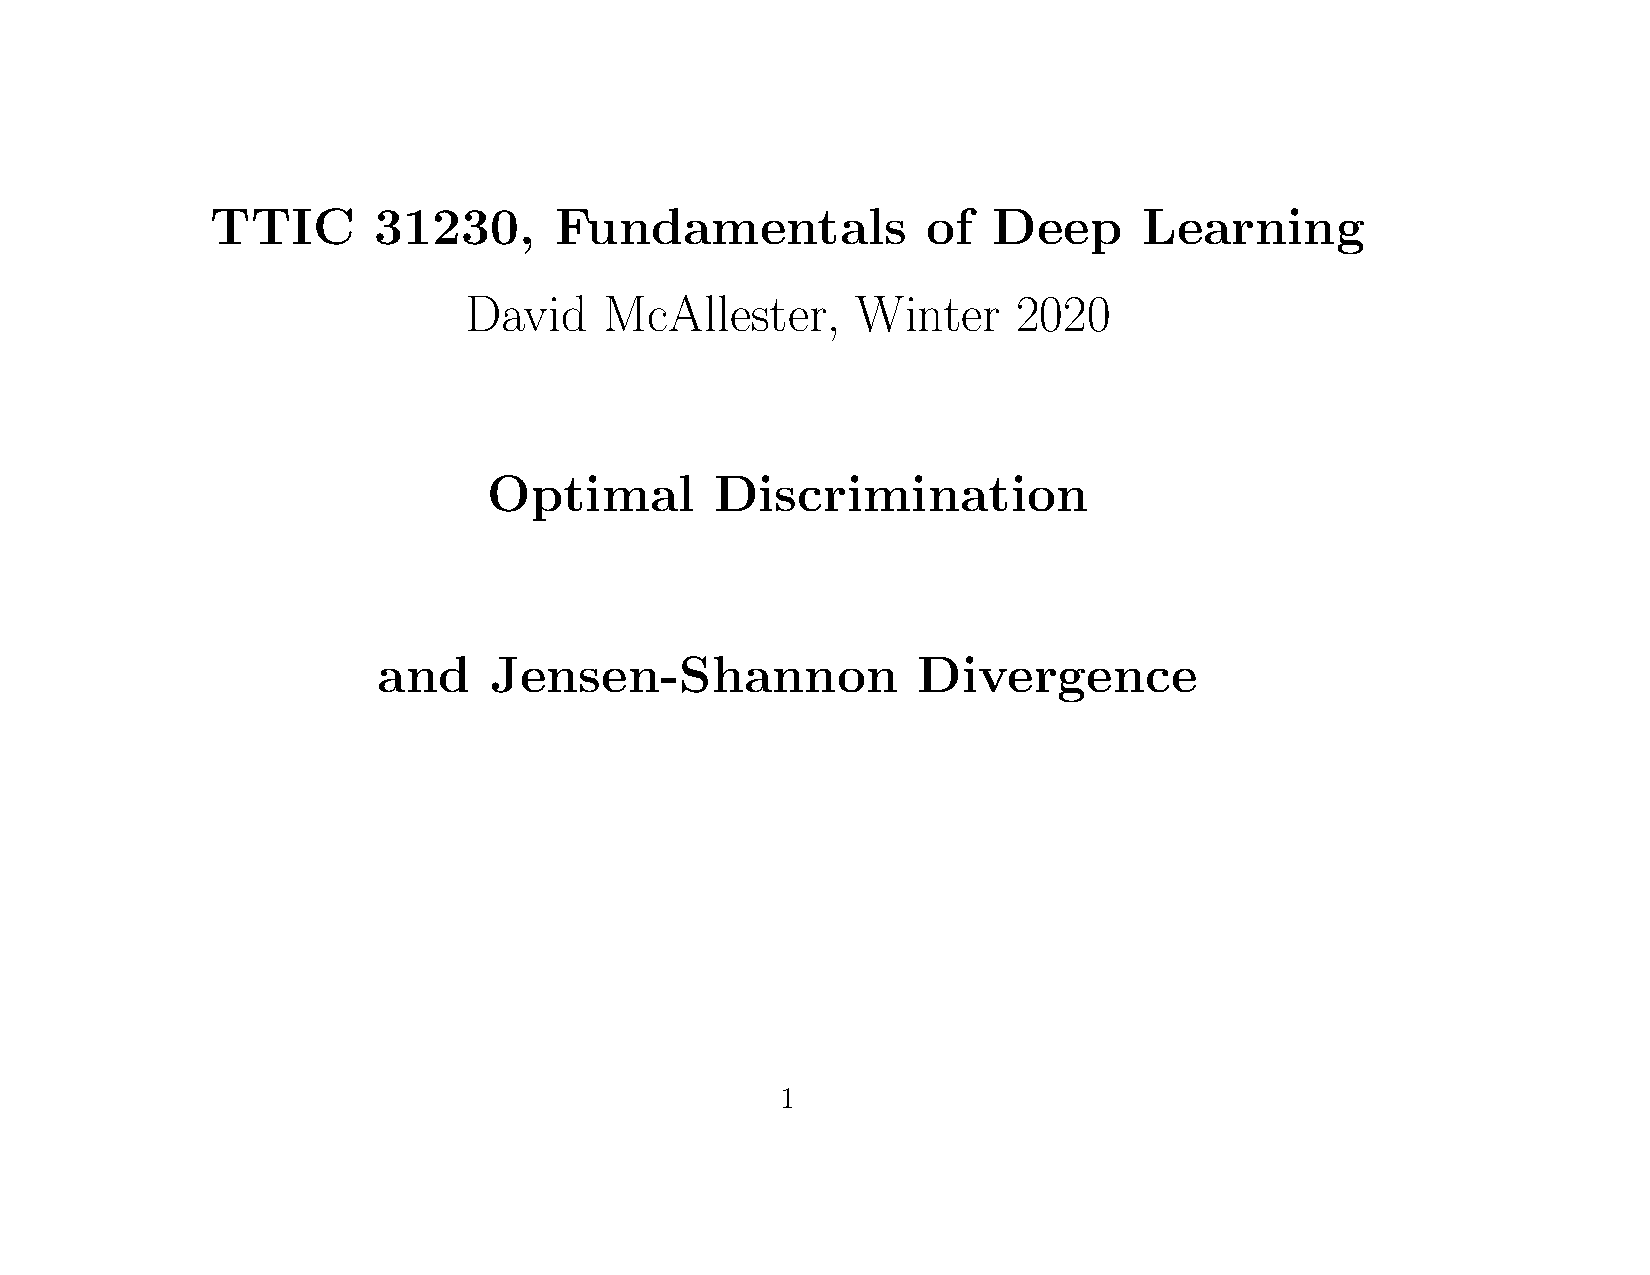
\includegraphics[height = 3.0in]{\images/Jensen}}

\vfill
For $f$ convex (upward curving) we have

\vfill
$$E[f(x)] \geq f(E[x])$$

\slide{Proving $KL(P,Q) \geq 0$}

\begin{eqnarray*}
  KL(P,Q) & = & \expectsub{y \sim P}{- \ln \frac{Q(y)}{P(y)}} \\
  \\
  & \geq & - \ln \expectsub{y\sim P}{\frac{Q(y)}{P(y)}} \\
  \\
  & = & - \ln \sum_y\; P(y) \frac{Q(y)}{P(y)}  \\
  \\
  & = & - \ln \sum_y Q(y) \\
  \\
  & = & 0
\end{eqnarray*}

\ignore{
\slideplain{Density Estimation}

Anything that can be done conditionally $P_\Phi(y|x)$ can also be done unconditionally $P_\Phi(y)$.

\vfill
We have unconditional cross-entropy training.

\begin{eqnarray*}
  \Phi^* & = & \argmin_\Phi \;\;E_{y \sim \mathrm{Pop}}  -\ln P_\Phi(y)
\end{eqnarray*}

\vfill
This is {\bf distribution modeling} or {\bf density estimation}.

\vfill
Density estimation is sometimes equated with {\bf unsupervised learning}.  A primary example is {\bf language modeling}.

\slide{Unsupervised Learning}

\centerline{\includegraphics[width = 8in]{\images/cake}}


\slide{Unsupervised Learning}

By ``unsupervised learning'' we will mean learning from {\bf massively available} data.  This is not a mathematical definition.

\vfill
{\bf Massive}: images, audio, text, video, click-through data.

\vfill
{\bf Less Massive}: car control data, stereo image pairs, closed captioned video, captioned images.

\vfill
{\bf Big}: Manually annotated images or audio.

\vfill
{\bf Small}: manually annotated text --- parse trees, named entities, semantic roles, coreference, entailment.

\vfill
{\bf Smallest:} Manually annotated text in an obscure language.

\slide{Colorization}

$$\Phi^* = \argmin_\Phi \expectsub{(x,y) \sim \mathrm{Pop}}{-\ln P_\Phi(y|x)}$$

\vfill
\centerline{\includegraphics[height=2in]{\images/Colorization}}

\vfill
We have massive data for colorization.

\vfill
Colorization is unsupervised structured labeling.
}


\slide{Appendix: The Rearrangement Trick}

\begin{eqnarray*}
KL(P,Q) & = & E_{x \sim P} \ln \;\frac{P(x)}{Q(x)} \\
\\
& = & E_{x \sim P} \left[(- \ln Q(x)) - (- \ln P(x))\right] \\
\\
& = & (E_{x\sim P} \;-\ln Q(x)) - (E_{x \sim P}\;-\ln P(x)) \\
\\
& = & H(P,Q) - H(P)
\end{eqnarray*}

\vfill
In general $E_{x \sim P} \;\ln \left(\prod_i A_i\right) = E_{x \sim P} \;\sum_i \ln A_i$ 


\slide{Summary}

{\color{red} $\Phi^* = \argmin_\Phi\;H(\pop,P_\Phi)$} unconditional

\vfill
{\color{red} $\Phi^* = \argmin_\Phi\;E_{x \sim \pop}\;H(\pop(y|x),P_\Phi(y|x))$} conditional

\vfill
\centerline{
  $\begin{array}{lrcl}
\mathrm{Entropy}: & {\color{red} H(P)} & = & {\color{red} E_{y \sim P}\;-\ln\;P(y)} \\
\\
\mathrm{Cross Entropy:} & {\color{red} H(P,Q)} & = & {\color{red} E_{y \sim P}\;-\ln\;Q(y)} \\
\\
\mathrm{KL\; Divergence:} & {\color{red} KL(P,Q)} & = & {\color{red} H(P,Q) - H(P)} \\
\\
& & = & {\color{red} E_{y \sim P}\;\;\; \ln\;\frac{P(y)}{Q(y)}}
\end{array}$}

\vfill
\centerline{{\color{red} $H(P,Q) \geq H(P),\;\;\;KL(P,Q) \geq 0,\;\;\;\argmin_Q\;H(P,Q) = P$}}


\ignore{
\slide{The Rearrangement Trick}

{\huge
\begin{eqnarray*}
H(P,Q) & \doteq & E_{x \sim P} \;-\ln Q(x) \\
\\
& = & E_{x \sim P}\; -\ln\;\left(P(x)\;\frac{Q(x)}{P(x)}\right) \\
\\
& = & E_{x\sim P}\; \left(-\ln P(x) + \ln \frac{P(x)}{Q(x)}\right) \\
\\
& = & \left(E_{x\sim P}\; -\ln P(x)\right) + \left(E_{x \sim P(x)} \ln \frac{P(x)}{Q(x)}\right) \\
\\
& = & H(P) + KL(P,Q) \\
\\
& \geq & H(P)
\end{eqnarray*}
}
}

\ignore{
\slideplain{Appendix: The Rearrangement Trick}

\begin{eqnarray*}
\mathrm{ELBO} & = & E_{z \sim P_\Psi(z|y)} \ln \;\frac{P_\Phi(z,y)}{P_\Psi(z|y)} \\
\\
\\
 & = & E_{z \sim P_\Psi(z|y)} \ln \;\frac{P_\Phi(z)P_\Phi(y|z)}{P_\Psi(z|y)} \\
\\
\\
 & = & E_{z \sim P_\Psi(z|y)} \ln \;\frac{P_\Phi(y)P_\Phi(z|y)}{P_\Psi(z|y)} \\
\end{eqnarray*}

\vfill
Each of the last two expressions can be grouped three different ways leading to six ways of writing the ELBO.}

\slideplain{END}

}
\end{document}
